\Chapter{Storing plot state of a game world}

% 1. Define plot
\section{Definition of plot state}

Because it is impossible to consider the various approaches to formalize the representation of the game's plot without taking into account the constraints, limitations and requirements of the game in question, evaluation scenarios are defined in regards to which the described methods are evaluated.

% 2. Define evaluation scenarios

\section{Evaluation scenarios}

\subsection{Scenario 1}

The player is tasked with solving a murder mystery in a closed space.
The gameplay loop consists of talking with non-playable characters and collecting clues.
There are three suspects, labeled A, B and C respectively.
The player must first obtain the first clue related to the weapon used by investigating the scene.
Then, during interviews they should obtain the clues relating to who possesses the weapon and who has a motive.
After that, the player might make an accusation and win the game.

In this scenario the player and characters are independent agents.
The scene is a special object that can be interacted with to gain the first clue.
The communication happens only between each character and the player and is uni-directional.
The list of possible clues is predefined.

\subsection{Scenario 2}

The player is tasked by a stall owner to steal a ring from the jewelery stall and plant it in another seller's pocket.
After the player does so, the stall owner yells for the guards to come arrest the thief.
If the ring is in the other seller's pocket, that seller will be considered the culprit and arrested.

In this scenario the player is able to interact with the task giver, the jeweler and the seller being framed.
The plot depends on the choices the player makes and the order they make them in.
If the player never plants the ring, the task giver will be punished for false accusation and will instead accuse the player.
If the player plants the ring in the pocket of the task giver, they will be the one arrested instead.
On the other hand, leaving the ring untouched and reporting to the task giver will cause the task giver to not be taken seriously as the jeweler will deny any theft taking place.

\subsection{Scenario 3}

The player overheard the general of enemy army talking about the plan to invade in three days.
They must reach the capital and inform the king of the danger to prepare the defensive.

This scenario is time sensitive and shows example of uni-directional interaction between the player and the enemy general.

\subsection{Scenario 4}

A dragon is seen flying from the mountains towards the forest.
The player is tasked with tracking it down.

Depending on where the player starts, they might or might not have witnessed the dragon themselves.
Through talking with the non-playable characters the player may find out who was a witness and who only heard about the dragon.
Based on the time of sighting, the player may deduce the direction of the dragon's flight.

% 3. Describe methods

\section{Methods}

All described scenarios are characterized by common elements.
They all refer to characters and the player as entities making decisions and performing actions.
In general, both the player and any non-playable characters can be called agents.
Each agent is independent from the rest and is able to act based on the subset of the plot available to them.
The actual implementation of each agent's behaviour can be as simple as a hardcoded line of dialogue and as complex as a set of rules enabling emergent behaviour.
Each method described below relates to the representation of the plot inside of the agent and not in the global sense of the whole game.
The differences in each method are related to what interactions can be modelled by it.

\subsection{SOAR}

One of the most important developments in the area of multi-agent systems and cognitive modelling was the SOAR (State, Operator, And Representation) cognitive architecture \cite{laird2019soar}.
It is a cognitive architecture that is designed to simulate human thinking and problem-solving processes.
At its core, SOAR is a symbolic, production-based system that uses rules to guide behavior.
This architecture consists of two major components:

\begin{itemize}
    \item Procedural memory (production memory) - set of production rules that can modify the state of the world and by extension, the state of the working memory by proposing operators
    \item Working memory - fact based knowledge represented by a symbolic graph structure describing the current state of the world
\end{itemize}

Many implementations of this architecture additionally include the concept of long-term memory structure that accumulates knowledge during the whole lifetime of the agent.
In general, implementation of the SOAR architecture can be called a production system.
Unlike many traditional production systems however, all rules that match against the current state of the world will fire (execute actions) in parallel.
This means that the list of rules is not ordered and conflicting operators may be proposed.
In such cases the usual strategy is to create a substate of the working memory with a new goal of conflict resolution.

The SOAR architecture has been successfuly utilized in creation of video game AI agents.
Examples include the application of this architecture to create an autonomous agent designed for playing Quake\cite{laird2001knows}, StarCraft\cite{turner2013soar-sc} and Descent 3\cite{van1999developing}.
Michael van Lent and John Laird in their work "Developing an Artificial Intelligence Engine"\cite{van1999developing} describe a decision cycle in an inference machine:

\begin{itemize}
    \item Perceive: Accept sensor information from the game
    \item Think: Select and execute relevant knowledge
    \item Act: Execute actions in the game
\end{itemize}

This cycle combined with the SOAR architecture allows for creation of a versatile agent capable of processing and propagating plot events in the game.
The first step allows the agent to modify the state of the working memory.
It can detect visible objects, including other agents and interactables such as containers, doors or even writings.
Then, the second step uses the working memory combined with production rules (procedural memory) to propose operators to execute.
Operators modify the state of the world, for example by moving the agent, taking the contents of a container, opening doors or interacting with another agent.
This constitutes the last step of the cycle and allows the agent to go back to the first step and update its working memory in preparation for the next step.

This architecture is versatile in that it can be used to model even very complex behaviours.
In order to avoid conflicts in the proposed operators by production rules that try to solve different goals, a goal token can be inserted into the working memory and used as a dependency in the production rules.
This way an agent may have a rule that changes the goal of the agent and thus modifies its next sequence of actions.

\subsection{Perceive}

The agent is equipped with simulated sensors that feed into its working memory.
These sensors interact with the simulated world and process the description of the world producing information that is then stored in the working memory of the agent.
Sensory information might include sight, hearing, sense of smell and other commonly thought of senses as well as abstract and arbitrary information that the agent can somehow perceive.
The combined information from all the sensors might produce information regarding the agent's awareness of the vicinity and the location of other agents in the simulated system as well as the state of the agent's body and own position in the game world.
The information is presented to the agent and it is up to the agent to decide what to do with it.
Sensors may only influence working memory of the agent.

\subsection{Think}

Agents have procedural memory that is represented by a collection of production rules that are executed in parallel.
Each rule might take as input an arbitrary set of working memory elements (WME), check arbitrary preconditions and produce arbitrary operators that when evaluated will change the state of the simulated world by means the agent's action.
While working memory is perfect for storing the immediate description of the agent's state, it is perhaps ill suited for storage of event based information elements.
For this reason the notion of long term memory is used for storage of facts characterized by timestamp of occurrence and description of the event.
Procedural memory and production rules therein may also utilize this storage to work with temporal data, for example to facilitate the agent remembering its travel trajectory or recording events such as successful executions of certain actions.
Procedural memory is usually immutable after creation of the agent but it is possible to store a production rule inside of working memory and by means of another production rule, modify the procedural memory adding the new rule to the bank of rules the agent possesses.
This can simulate agent learning new inference rules and behaviours, for example through reading a book or being taught by other agent.

\subsection{Act}

The act of action when performed by the simulated agent is represented by an operator being evaluated.
An operator represents an action that an agent wishes to perform.
The game world is in charge of evaluating the results of the operator and rejecting it in case the agent is not allowed to perform it due to any condition that the agent itself is not aware of.
Because production rules are executed in parallel and thus output multiple operators, it is possible for conflicts to occur.
A single agent may think to move forward and back at the same time.
Because the order in which actions are performed may impact the result, it is important to define a conflict resolution strategy, either for each agent or for the whole game in general.
Such a strategy does not need to necessarily be deterministic as usually it is impossible to determine which operator should take precedence and defining conflict resolution policies for each possible set of conflicting operators is often not a viable approach.
One example of a conflict resolution strategy is a strategy that chooses a random order for conflicting operators and executes them until one is accepted.
This shows the second part of the problem which is conflict detection.
Any two operators can be conflicting in terms of resulting state of the game world.
The simplest approach is not allowing the agent to execute multiple operators at the same time and instead force it to choose one specific action instead.

\subsection{Interactions}

An agent might lack the sense of vision and instead start with its known position WME at coordinates $v_0=(0, 0)$.
It wishes to progress forward (positive $y$ axis) and so proposes the operator $Move(Agent, 0, 1)$ via a production rule with constant output.
The game world accepts the operator, evaluates it and the agent is then made aware of the operator's successful execution.
The agent now has the position WME set to $v=(0, 1)$.
It proposes the same operator again.
This time the game world rejects the action because of a wall that stands at $v=(0, 2)$.
The agent did not modify its position WME this time but added a second WME $WallAt(0, 2)$.
A production rule exists that checks if there is a $WallAt$ WME directly ahead of the current position and if so, produces operator $Move(Agent, 1, 0)$.
The production rule that produces the constant $Move(Agent, 0, 1)$ operator fires as well and afterwards the agent needs to decide which action to take.
The agent has a conflict resolution strategy defined as:

\begin{itemize}
    \item choose random
    \item fallback when action rejected
\end{itemize}

This policy means that either the lateral move will be selected by random chance or the previous operator will be selected, evaluated, subsequently rejected and a fallback would occurr to the next one.
This example shows that a virtual agent possesses a limited capacity to learn and build the information bank describing the state of the world around it.
In some implementations, the immediate position of the agent would be stored as WME while the position of each discovered wall would be put in long-term memory.

% \subsection{Event Calculus}

% The two most commonly used formalism for representation of plot state in games are situation calculus and event calculus.
% The situation calculus is a logical language for representing changes\cite{lin2008situation}.
% According to Levesque, in situation calculus "the foundational axioms for situations provide a purely qualitative notion of time whose only temporal concept is sequential action occurrence: an action occurs before or after another within"\cite{levesque1998foundations}.
% The event calculus is a formalism for reasoning about action and change \cite{mueller2008event}.
% Similarly to the situation calculus, the event calculus uses the concept of actions (called "events") and fluents.
% The main difference is that events can be external and happen at specific time points which makes it essential for modelling plot state where a plot event can happen in isolation.
% Event calculus was introduced first in 1986 by Kowalski and Sergot \cite{kowalski1986logic}.
% It was then simplified in 1992 \cite{kakas1992abductive}.
% In general, the ontology of event calculus includes the definitions of fluents and actions.
% In order to utilize event calculus in representation of plot points, one can limit the type of fluents to just propositional fluents.
% The predicates used to model plot state are described in table \ref{tab:event-calculus-predicates}.

% \begin{table}[]
%     \centering
%     \begin{tabular}{@{}ll@{}}
%         \toprule
%         Predicate                                       & Meaning                                                            \\ \midrule
%         $Initially_P \left( \beta \right)$              & Fluent $\beta$ holds from $\tau_0$                                 \\
%         $Initiates \left( \alpha, \beta, \tau \right)$  & Fluent $\beta$ starts to hold after action $\alpha$ at time $\tau$ \\
%         $Terminates \left( \alpha, \beta, \tau \right)$ & Fluent $\beta$ stops holding after action $\alpha$ at time $\tau$  \\
%         $Happens \left( \alpha, \tau \right)$           & Action $\alpha$ occurs at time $\tau$                              \\
%         $HoldsAt \left( \beta, \tau \right)$            & Fluent $\beta$ holds at time $\tau$                                \\
%         $Clipped \left( \tau_1, \beta, \tau_2 \right)$  & Fluent $\beta$ is terminated between times $\tau_1$ and $\tau_2$   \\
%         $\tau_1 < \tau_2$                               & Time point $\tau_1$ is before time point $\tau_2$                  \\ \bottomrule
%     \end{tabular}
%     \caption{Event calculus predicates used to express plot state, based on Shanahan et al.\cite{shanahan2001event}}
%     \label{tab:event-calculus-predicates}
% \end{table}

% Additionally some implicit axioms need to be defined to ensure uniqueness of names for fluents and actions as well as the common sense law of inertia for fluents.
% The latter implies that fluents do not change unless given reason to.
% Advanced variants of event calculus allow for releasing of fluents from this constraint and thus effectivelly making them become undefined unless explicitly stated.
% The application of event calculus in representation and simulation of plot state can be divided into two distinct use cases.
% The first use case is to represent the state of the plot at any given time as an array of fluents with their calculated value at the given time.
% The second one is mutation of the plot state via actions that influence the fluents.
% Because the plot state is not global and insted exists only within each individual agent as a very small subset of the whole plot, the actions influence only the fluents known by the agent perciving them.
% It is assumed that an action that happened but was not percived by anyone is of no consequence.
% A king dieing in his bedchambers does not affect the plot unless he is discovered to be dead.
% At that moment, the action that changed the state of the plot was not the death itself but rather its discovery.
% This distinction allows for separation of the concept of global plot which is the sum of all agents' actions and knowledge and the local plot which exists individually for each agent.
% A player is similarly such an agent in a system with the difference that while they may also be used for simulation purposes, the human observer is additionally perceiving the plot and forming their own local plot state in their head.
% Table \ref{tab:event-calculus-plot-predicates} defines additional extensions to event calculus which enable representation of knowledge by the agents.

% \begin{table}[]
%     \centering
%     \begin{tabular}{@{}ll@{}}
%         \toprule
%         Predicate                               & Meaning                                                         \\ \midrule
%         $Known_P \left( A, \beta, \tau \right)$ & agent $A$ knows fluent $\beta$ held at time $\tau$              \\
%         $Known_N \left( A, \beta, \tau \right)$ & agent $A$ knows fluent $\beta$ did not hold at time $\tau$      \\
%         $Record \left( A, \beta, \tau \right)$  & agent $A$ records state of fluent $\beta$ at the time of $\tau$ \\ \bottomrule
%     \end{tabular}
%     \caption{Extension to event calculus enabling plot representation}
%     \label{tab:event-calculus-plot-predicates}
% \end{table}

% In order to represent an example of a plot event defined within this framework, the death of a king might be used.
% For this, a set of fluents and actions need to be defined first.

% \begin{equation}
%     Initially \left( KingAlive \right)
% \end{equation}

% \begin{equation}
%     Terminates \left( DrinkPoison, KingAlive, t \right) \Leftarrow HoldsAt \left( KingAlive, t \right)
% \end{equation}

% \begin{equation}
%     Known_N \left( A, \lnot \beta, t \right) \Leftarrow Record \left( A, \lnot \beta, t \right)
% \end{equation}

% Finally, a narrative looks like so:

% \begin{equation}
%     Happens \left( DrinkPoison, T_1 \right)
% \end{equation}

% \begin{equation}
%     \label{eqn:servant-saw-kind-dead}
%     Record \left( Servant, \lnot KingAlive, T_2 \right)
% \end{equation}

% \begin{equation}
%     T_1 < T_2
% \end{equation}

% After \ref{eqn:servant-saw-kind-dead} the fluent $Known_N \left( Servant, KingAlive, T_2 \right)$ holds which means that the servant witnessed the king being dead and knows only as much as to be able to tell that he was dead since $T_2$.

% In general, plot state of a game world can be represented in a plethora of ways, depending on the defined use cases.
% Plot state can be associated with the state of knowledge in a given region or with an individual agent.
% The first approach is used for spatial modelling where the game world is partitioned into disjoint regions that can be considered to be homogeneus in terms of their reaction to various kinds of plot events.
% The second approach is useful for creation of logical models that may be employed to simulate very precise and complex interactions between individual agents.
% It is worth mentioning that an agent does not necessarily need to be a representation of a person but may as well be a whole region, a city, a town or even an abstract concept.
% Spatial models are well suited for simulating how a given plot even will impact the rest of the game world in terms in terms of information propagation.
% Logical models excel in representing complex interactions and simulating how agents relay information about plot events to each other and thus gain knowledge on the state of the plot state in the game world.

% While event calculus can model any narrative in a consistent way, its limitations are exposed when one starts to find ways to apply it in a distributed system of agents and interactions.
% Each agent can have their own version of the narrative and thus their own individual system of fluents and their states.
% This means that for one agent the fluent $KingAlive$ may hold while for another agent it may not.
% There can be many reasons for this state of the plot.
% The second agent may have just been a witness to the death of the king or they may simply not be aware of the king's existence in the first place.
% When two agents in such a system interact with eachother, they might share their knowledge and exchange information on the fluents that they are aware of.
% In trivial cases this can mean an agent giving the second agent a predicate $Initiates \left( \alpha, \beta, \tau \right)$ to make the fluent hold since some moment in time $\tau$ or termining an already holding fluent via the predicate $Terminates \left( \alpha, \beta, \tau \right)$.
% This approach has the same pitfalls as distributed systems and event ordering algorithms used therein \cite{lamport2019time}.
% Figure \ref{fig:temporal_conflicts_in_event_exchange} shows how different situations may be handled in a system based solely on event calculus.
% The exact results depend on the exact implementation of the event exchange mechanism for a pair of agents.

% \begin{figure}
%     \centering
%     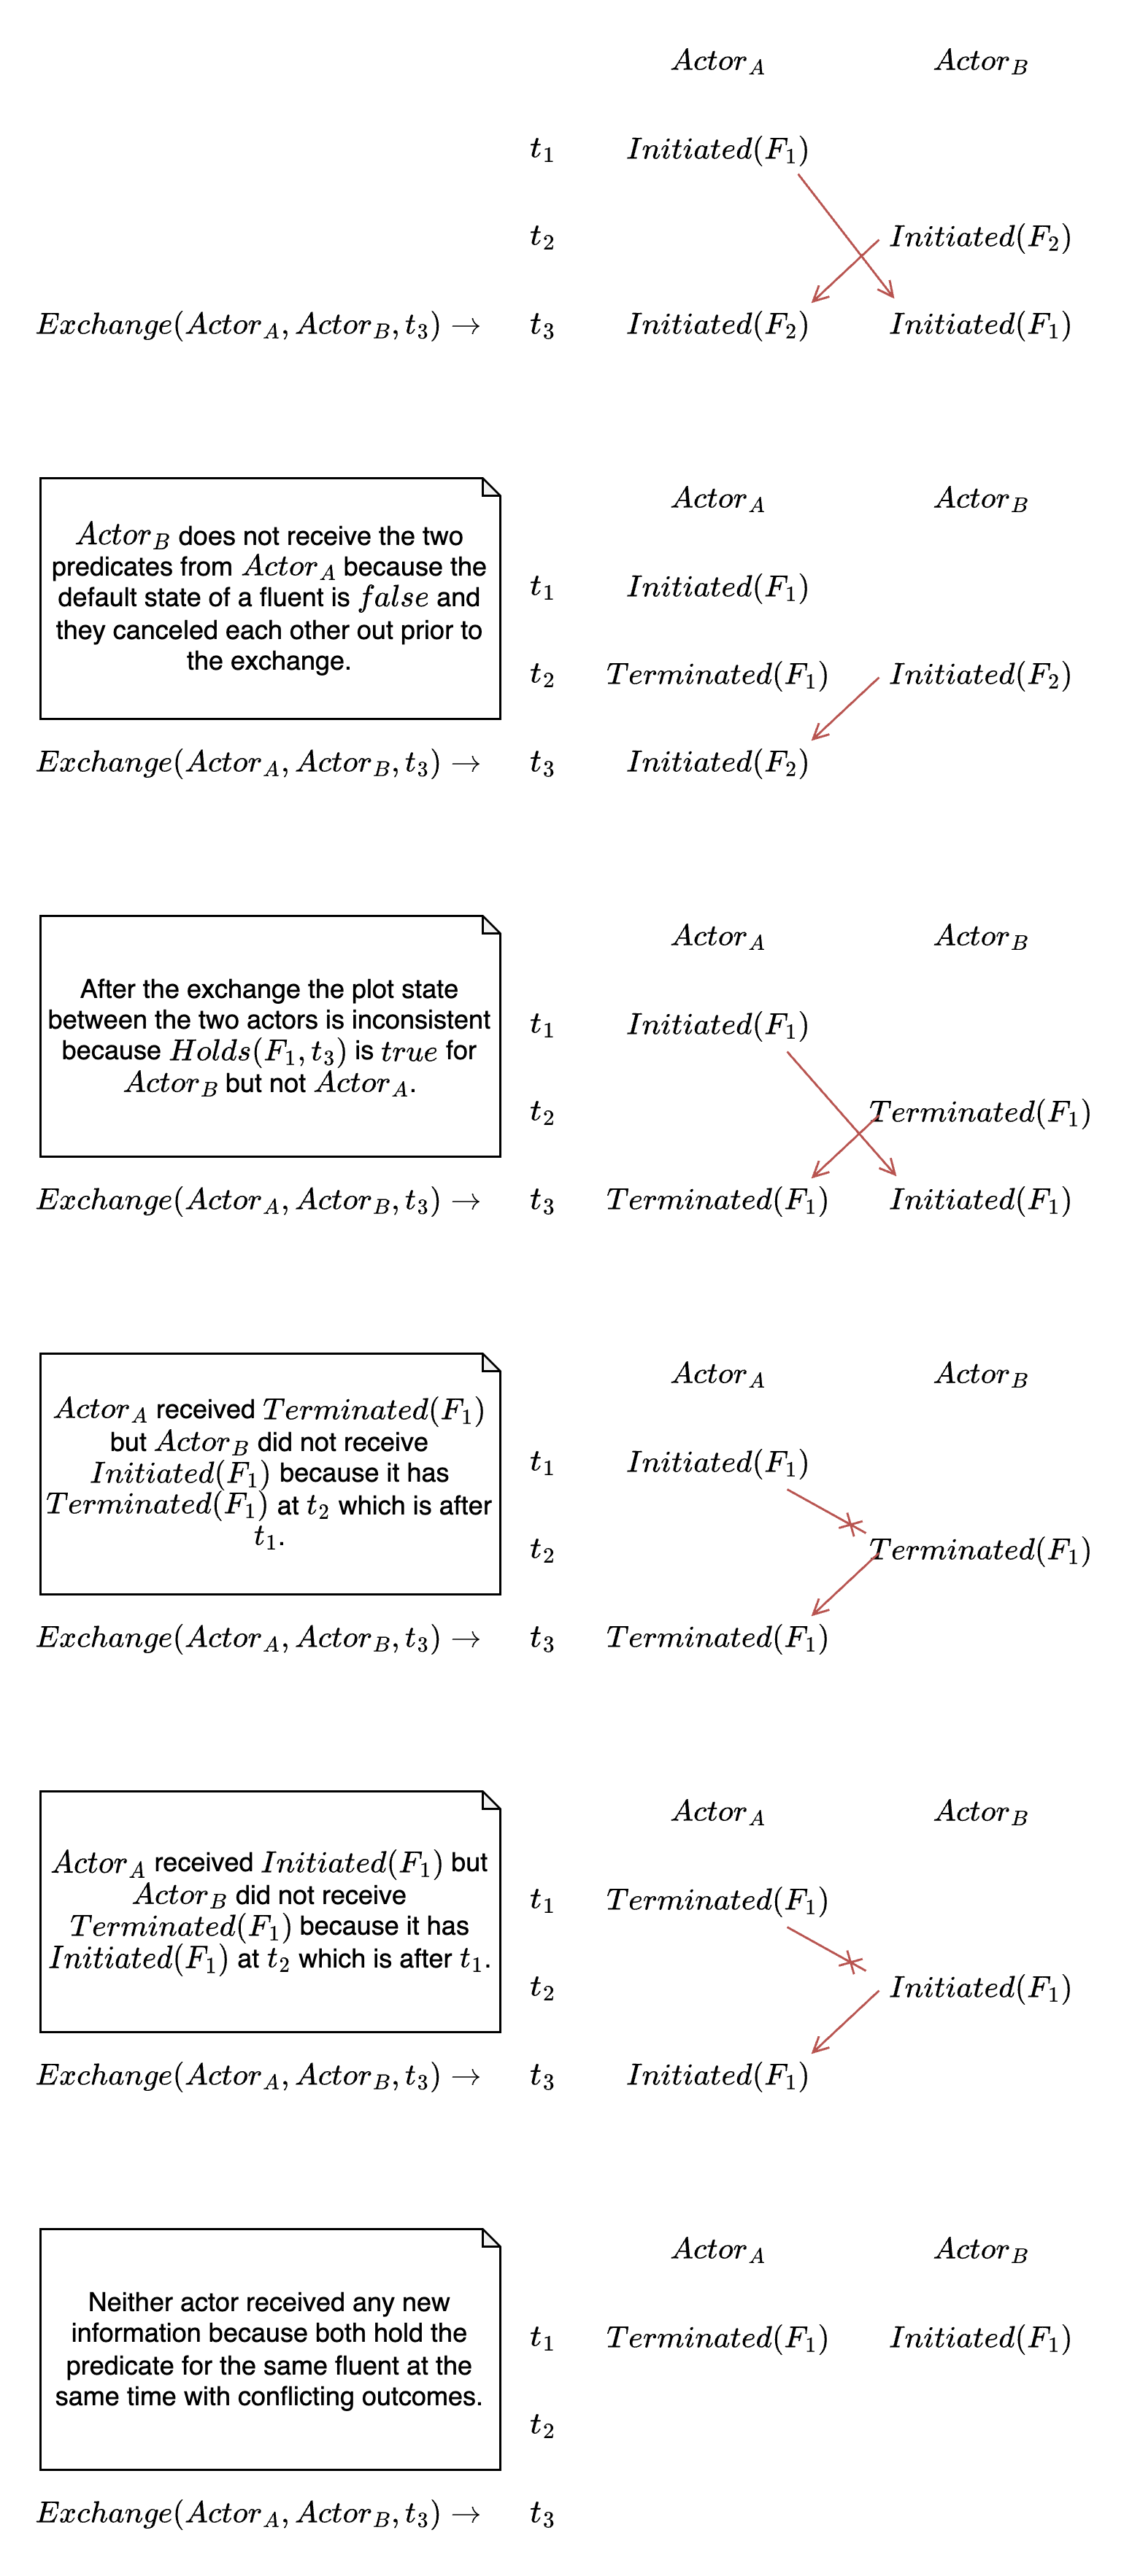
\includegraphics[width=0.55\textwidth]{images/temporal_conflicts_in_event_exchange.drawio.png}
%     \caption{Selected outcomes of event exchange between two agents with description of possible conflicts}
%     \label{fig:temporal_conflicts_in_event_exchange}
% \end{figure}

% The problems described above matter only in the case of games where there will be two agents exchanging plot state simultaneously.
% Not all games have this requirement and those that do not, that is those with unidirectional information exchange mechanisms, will inherently be free from these pitfalls.
% Similarly, some games do not require deterministic state of the plot or the ability for an agent to forget information.
% In these types of games, event calculus might not be applicable and other solutions should be considered.

% \subsection {Inference rules}

% The best approach in choosing the framework for representing plot state depends on the type of plot to be represented and the intended game mechanics.
% An RPG game where the player can freely interact with the simulated world will have a different set of requirements than a murder mystery game.
% The latter may be satisfied with a probabilistic or confidence-based approach and have no need for actions and instead require inference rules.
% In such case the player is usually tasked with solving a mystery based on a set of clues.
% In a regular game the solution to the mystery is usually predetermined or semi-random but in general singular per game.
% Using a confidence or probabilistic approach, the game may accept any solution as long as the probability for it being correct is above a certain defined threshold.
% The concepts of fluents may be borrowed from event calculus to represent individual clues.
% For example consider the game as previously described.
% The goal of the game is to aquire the fluent $IsCulprit \left( Suspect_N \right)$ where $N$ is the number of the suspect that committed the crime.
% The clues in the game are $HasWeapon \left( Suspect_N \right)$ and $HasMotive \left( Suspect_N \right)$.

% \begin{equation}
%     \label{eqn:weapon_motive_inference}
%     HasWeapon \left( Suspect_N \right) \land HasMotive \left( Suspect_N \right) \Rightarrow  IsCulprit \left( Suspect_N \right)
% \end{equation}

% There is one inference rule defined in equation \ref{eqn:weapon_motive_inference}.
% Consider the state of the game where there are three agents $Suspect_A$, $Suspect_B$, $Suspect_C$.
% The player can hold a conversation with each of them.
% Each conversation yields different clues.

% \begin{equation}
%     Suspect_A \rightarrow HasWeapon \left( Suspect_B \right) \land HasMotive \left( Suspect_C \right)
% \end{equation}

% \begin{equation}
%     Suspect_B \rightarrow HasMotive \left( Suspect_C \right) \land HasWeapon \left( Suspect_A \right)
% \end{equation}

% \begin{equation}
%     Suspect_C \rightarrow HasMotive \left( Suspect_B \right)
% \end{equation}

% Based on the inference rule defined for $IsCulprit$ one can get:

% \begin{equation}
%     HasWeapon \left( Suspect_B \right) \land HasMotive \left( Suspect_B \right) \Rightarrow  IsCulprit \left( Suspect_B \right)
% \end{equation}

% This is fine until $Suspect_C$ divulges that $HasMotive \left( Suspect_A \right)$.
% After this the following holds:

% \begin{equation}
%     IsCulprit \left( Suspect_A \right) \land IsCulprit \left( Suspect_B \right)
% \end{equation}

% \subsection{Confidence/probability based inference}

% Under the assumption that there is exactly a single culprit, the probabilistic approach can be taken.
% Probability function $P(X)$ can be defined for each fluent.

% \begin{equation}
%     \label{eqn:is_culprit_probability_pre}
%     P \left( IsCulprit \left( Suspect_A \right) \right) + P \left( IsCulprit \left( Suspect_B \right) \right) + P \left( IsCulprit \left( Suspect_C \right) \right) = 1
% \end{equation}

% Because there is no way to attain $IsCulprit \left( Suspect_C \right)$, its probability will be equal to zero and so \ref{eqn:is_culprit_probability_pre} becomes \ref{eqn:is_culprit_probability_post}.

% \begin{equation}
%     \label{eqn:is_culprit_probability_post}
%     P \left( IsCulprit \left( Suspect_A \right) \right) + P \left( IsCulprit \left( Suspect_B \right) \right) = 1
% \end{equation}

% So far however each outcome is equally probable and there is no way to determine the probability of any suspect being the culprit based on the clues themselves.

% 4. Compare methods
% 5. Present conclusions

% Plot events: 
% Śmierć władcy rozprzestrzeni się od punktu centralnego wzdłuż dróg
% Wybuch wulkanu rozprzetrzeni się od każdego miejsca z którego był widoczny
% Smok będzie widziany na całej jego trasie lotu, uwzględniając czas.
% Epidemia, każdy nowy chory ma większy priorytet

% \section{Partitioning of agents to form spatial models}

% Spatial models can be constructed by partitioning a logical model after assigning each agent its physical location and calculating bounds of each logical network.
% This method requires that agents form disjoint sets of information networks.
% Any plot even propagated to each spatial region can be either made immedietely accessible to all members of the embedded logical model or to a specific subset of agents.
% Similarly an agent may be designated a gateway out of the logical model into the spatial one and gain the ability to propagate information to other spatial regions.
% This way a game world may employ both types of models to essentially store the whole plot state and simulate in detail only the subset of regions that the player is in close proximity to.
% This approach makes usage of the logical model a viable solution for large scale open world games.

% \section{Difference between knowledge and information}

% % What is information?
% The most important distinction when building information propagation models is the one that differentiates knowledge from information.
% The latter can be propagated while the former cannot.
% This is due to the fact that information represents a statement of fact, irrespective of whether it is true or not.
% A claim that people with axes are walking down the road towards the forest can be an information.
% It should be considered to be fundamentally literal and represent nothing more than the messaging mechanism used to convey it.

% % Knowledge
% A person has a mind capable of linking events, seeing connections between facts, identifying patterns and inferring new knowledge from received information.
% Anyone can easily see that such a group of aforementioned people can represent lumberjacks aiming to chop down the trees.
% Note that neither the word lumberjack or the act of chopping down any tree was mentioned before.
% This shows the distinction between what is pure information and what can be considered knowledge.
% After all, how does one come to the conclusion that axes and trees must mean lumberjacks?
% One needs to be aware of the concept of an axe and its function as well as the existence of the trade of forestry to make that connection.

% % Propagation
% After realizing the meaning of people with axes going towards a forest, one can decide to tell others of this news by formulating a new statement of fact: "Lumberjacks are going to the forest".
% A more natural example would be a person telling a friend that someone told them about a group of lumberjacks heading to a forest.
% This is an example of information propagation.
% It can be illustrated more clearly by assuming the person who heard about the people heading towards the forest had recently seen a pack of wolves in the area.
% They might get alarmed and wish to warn the unsuspecting workers.
% The information "there are wolves in the forest" has the characteristic of urgency as well as importance.
% It is urgent because telling it after the workers get to the forest misses the whole point of warning them.
% It is important because it influences their safety.
% These two fagents lay the foundation for best possible propagation effect.
% One would immedietely embark on a trip to warn the lumberjacks of the dangers lurking in the forest and probably mention the situation to anyone they pass by.
% This particular situation also has the characteristic of being targeted towards a specific group.

% % TODO: Find characteristics of information in literature
% % Information characteristics
% Information can be urgent, important and have a target group of receiving people.
% Urgency determines the temporal aspect of propagation.
% Importance influences how much effort one is willing to spend delivering the information.
% A target audience limits the list of potential receivers.
% An information can be urgent and not important, that would simply mean that it will expire after some limited time but if the effort to deliver it on time is too great, it is possible that it won't be done.
% It can be important but not urgent just as well.
% In this case it means that it must be delivered but there are no consequences to doing so later rather than sooner.
% It is worth noting however that importance also influences the temporal element of information propagation as more important messages are going to be propagated faster.
% A target audience can be homogeneus (a group of lumberjacks) or have a variety of different people.
% A person doing the propagation can have a list of intended recipents of a message they are carrying.
% There can also be people who are subscribers of selected kinds of information.
% A mother would like to know if anything happens to her child and as such one can say she subscribes information regarding the health of her children.
% In real life there are many more aspects and characteristcs that are deeper and more nuanced that what was described.
% No artifical model can represent accurately the intricacies of the human mind, much less a group of minds.

% % How information and knowledge interact
% Information cannot exist without someone to perceive it and knowledge cannot exist without information.
% Whenever there is some entity that is able to receive information and understand it, it can produce knowledge.
% Information nececessitates a receiver to exist somewhere in the system that can produce knowledge.
% This means that all three must always be present.
% Collections of agents able to receive information and process it into knowledge as well as create new information and share it with other agents will be henceforth reffered to as information systems.

% % Complexity of information systems
% An information system is a set of agents possessing knowledge and wishing to spread it in the form of information.
% Because the complexity of real information systems is too great, simplification needs to be made in order to focus on the important aspects of such a system.
% The key elements of any information system can be identified:
% \begin{itemize}
%     \item agent - a person capable of processing information, holds knowledge and can produce new information
%     \item Information - statement originating from any information source, ie. an agent
%     \item Information source - any source of information, can be an agent or an inanimate source such as a recording or text
%     \item Information pathway - any link between agents through which information can travel, can affect the information causing distortion or impact the propagation
% \end{itemize}
% agents may be offered information or they might produce information themselves.
% This must always happen through an information pathway.
% Inanimate sources of information, ie a written book, may exist within the same system and are considered to be always producing some (usually constant) information.
% An agent may react differently when offered different kinds of information or even the same one repeatedly.
% To illustrate that one can imagine being interested in buying a new pair of shoes if seeing the advertisment of them for the first time and getting more annoyed each consecutive time the same advertisment is played.
% % TODO: Cite the work modelling marketing strategy effectiveness
% This behaviour is usually the target of marketing strategy analysis as simply increasing the intensiveness of advertisment broadcast will not increase the demand for the shown product.
% Aside from being able to receive information, an agent may decide to share it with other agents.
% They might decide to choose a target group or broadcast it to everyone they can reach.
% Some agents may seek certain types of information and query for it anytime they can.
% In order to do so, agents must possess some knowledge.

% % Complexity of knowledge
% Knowledge is a set of statements about the world that are consistent (irrespective of truthfulness).
% One can claim that the planet is flat while another person might disagree and it is valid to say that both possess knowledge about the shape of the world.
% A person can then infer new facts on the basis of what they already know and for instance make a claim that travelling past the edge of the Earth will cause the daring explorer to fall to their demise.
% The second person will then receive such information and basing on their opposing set of known statements will reject it and possibly reduce the opinion of the first person, being less likely to believe anything they might then tell them.
% It is however impossible to model the interactions between information necessary to infer new information the same way that happens in the human mind, at the very least not in any feasible way.
% The complexity of interconnectedness of knowledge and information alike is too great to be represented fully.
% One can however make assumptions and put constraints on the type of statements allowed and the knowledge that can be gained and thus create a simplistic representation of an information system.

% % Scope - logical vs spatial
% There are two main types of information systems that can be used to model information propagation:
% % TODO: Add some citation to "podział przestrzeni na abstrakcyjną i fizyczną"
% \begin{itemize}
%     \item spatial - they model information spread across space, usually partitioned into homogeneus segments or tiles
%     \item logical - representing connections between agents without taking into account physical relationships between them
% \end{itemize}
% The first kind of information system, spatial information systems (SIS) can be used to model large scale events happening across the world.
% The most important assumption in these kind of systems is the homogenuity of any given unit of space as defined by the chosen partitioning method.
% They assume that information has some kind of physical propagation characteristic that allows it to travel across space.
% In these systems an agent needs not to be represented individually but rather can be treated as part of a homogeneus group.
% This model might be used to represent how news regarding the death of a ruler might spread from the captial to the most remote villages.
% The second type of information systems, logical information systerms (LIS) work on the basis of individual agents and interactions between them.
% They are ill suited for large scale modelling as the number of agents to be considered would grow considerably.
% Of course, a spatial system can be represented as a logical system if some of the more important regions of the spatial model are chosen and represented as agents in the logical model.

% % What does it mean for information to be considered as propagated?
% The process of propagating information from one agent to another can be considered in the scope of physical information receival as well as logical aspect of interpretation.
% The act of knowledge assimilation is inherently present in the process of agent receiving information from any external source.
% % Is it sufficient to transfer information from source to target?
% Information can reach its target in a plethora of ways.
% In many models
% % What happens after information reaches the target?
% % What are the sources of information?



